\section{Post-Training Data Collection}
\label{sec:post-training-data}

\subsection{Agentic Coding}
\label{sec:agentic-coding-data}

We collect post-training data for agentic coding across three complementary domains: software engineering (SWE), application development (AppDev), and terminal interaction tasks, covering repository-level code evolution, full-stack development, and interactive terminal environments.

% To enable agentic coding in real-world software development scenarios, we focus on three core principles: scalability, diversity, and verifiability. These principles guide the collection, synthesis, and validation of tasks to ensure that the resulting training data is large-scale, varied, and reliably executable. We apply these principles across two complementary domains: Software Engineering (SWE) tasks and Application Development (AppDev) tasks, representing code evolution and full-stack system development, respectively.

\begin{figure}[h]
\centering
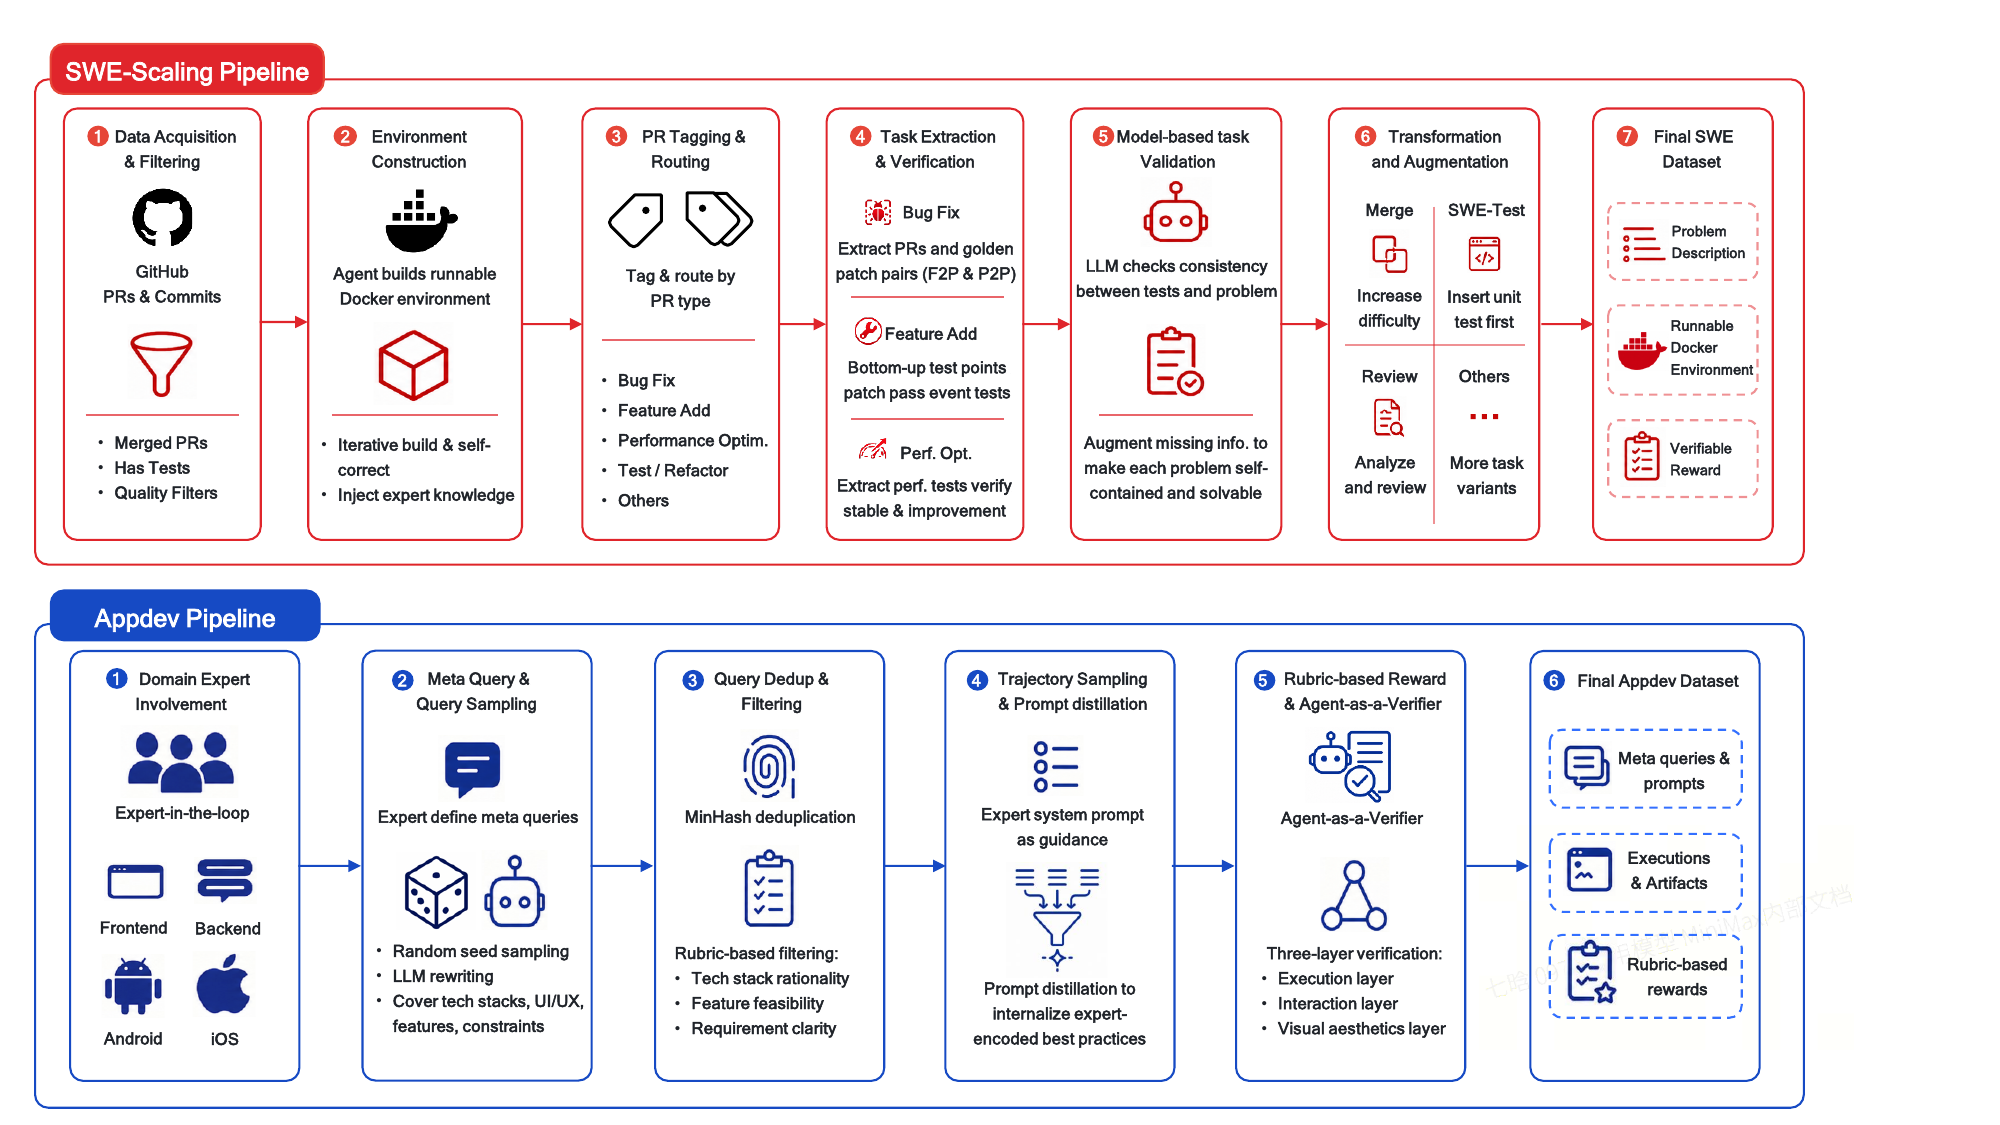
\includegraphics[width=\textwidth]{figures_new/swe_appdev.pdf}
\caption{The agentic coding data pipelines for SWE and AppDev tasks.}
\label{fig:swe-appdev}
\end{figure}

\subsubsection{Real-Data Driven Collection: Software Engineering Tasks}

Constructing training data for coding agents poses three coupled challenges: achieving broad task diversity, ensuring objective verifiability, and scaling to the volumes that large-scale training demands. GitHub serves as a rich and naturally structured source for collecting such data: a well-structured pull request captures a description, associated code changes, and test cases that provide objective correctness signals. However, raw PR data is inherently noisy and cannot be used directly, motivating our construction of a real-data driven SWE-scaling pipeline: an agent-driven automated data pipeline based on raw GitHub data to produce diverse, verifiable SWE-style datasets and environments. Specifically, the pipeline proceeds through the following six consecutive stages.

\begin{itemize}
    \item \textbf{PR collection and filtering.} The first stage of the pipeline involves large-scale crawling of public GitHub repositories with permissive licenses to collect pull requests and their linked issues, which together provide code diffs, test files, and problem statements. Since raw GitHub data is inherently noisy, we apply a rule-based quality filter on the PRs that were eventually merged, along with additional criteria such as the presence of relevant test cases.

    \item \textbf{Agent-synthesized multi-language Docker environments.} In the SWE-scaling pipeline, we aim to construct a runnable Docker environment for each PR.
    However, we observe that environment synthesis is less reliable in non-Python settings due to heterogeneous dependencies and version conflicts. To address this, we introduce an agent-driven execution loop that incorporates expert knowledge, enabling iterative generation and refinement of build scripts guided by execution feedback. The key dimensions we address are as follows:

    \begin{itemize}
        \item \textit{Build system orchestration in compiled languages.} Compiled languages such as Java, Go, Rust, and C++ require complex toolchain coordination, including compiler versions, build tools, and dependency resolution.
    
        \item \textit{Heterogeneous execution and testing interfaces.} Different languages expose distinct build and testing pipelines, requiring unified yet adaptable execution interfaces for environment setup and validation.
    
        \item \textit{Repository-level structural variability.} Differences in project organization and dependency specification across repositories necessitate adaptive strategies for code localization and test execution.
    \end{itemize}


    % \begin{itemize}
    %     \item \textit{Environmental complexity of compiled languages.} Python, as an interpreted language, has relatively simple configuration. However, for compiled languages like Java, Go, Rust, and C++, we need to handle complex compilation toolchains, version compatibility, and cross-compilation issues. A Java project might depend on a specific version of JDK, Maven/Gradle, and numerous third-party libraries; an error in any link can lead to build failure.
    %     \item \textit{Diverse test frameworks.} In the Python ecosystem, pytest dominates, but test frameworks in other languages are more fragmented. Java has JUnit and TestNG; JavaScript has Jest, Mocha, and Vitest; Go has the built-in testing package but also extensions like \texttt{testify}; Rust has built-in tests and \texttt{criterion}, etc. We need to design specialized test execution and result parsing logic for each framework.
    %     \item \textit{Dependency management and project structure.} Package managers for different languages differ vastly in dependency resolution, version locking, and private repository support. The nested structure of npm's \texttt{node\_modules}, Maven's central repository mechanism, and Cargo's semantic versioning all require targeted handling. Simultaneously, project structure standards vary: Python structures are flexible, but Java projects usually follow strict Maven/Gradle directory standards; Go projects have GOPATH and Go Modules modes; Rust projects have the concept of a workspace. Understanding these dependency management mechanisms and project structures is crucial for correctly locating code and running tests.
    %     \item \textit{Difficulty in parsing error messages.} Error message formats produced by different languages and toolchains vary widely; compile errors, link errors, and runtime errors also manifest differently. We need to train the model to understand these diverse error messages and extract useful debugging clues from them.
    % \end{itemize}


    \item \textbf{PR tagging and task diversification.} After constructing the Docker environment for each PR, we perform PR-level tagging and routing. GitHub PRs span a broad taxonomy of task types, including bug fixes, feature additions, performance optimizations, refactoring, and test construction. Such routing is necessary because different task types require distinct formulations of downstream verifiable rewards.
    

    \item \textbf{Test-based verifiable reward construction.} We design task-specific reward functions grounded in test-case execution, as different PR types require fundamentally different evaluation criteria.

    \begin{itemize}
        \item \textit{Bug fix.} For bug-fix scenarios, we extract F2P (Fail-to-Pass) and P2P (Pass-to-Pass) test cases. If a golden patch passes these tests, the data is considered valid. We then let the model act as an agent to fix the bug in a sandbox and verify correctness using both F2P and P2P tests. P2P tests are particularly important to ensure that no new bugs are introduced during the fix.
        
        \item \textit{Feature addition.} For feature additions, traditional F2P/P2P logic may not apply, since tests often depend on newly introduced code. Instead, we focus on extracting newly added test points and ensuring the golden patch passes them.
        
        \item \textit{Performance optimization.} Since performance optimization has no bug-fixing process, in such cases we extract P2P tests that can verify stable and significant performance differences before and after the optimization.
    \end{itemize}


    \item \textbf{Model-based task validation.} Raw GitHub PRs are often weakly structured, and their associated test cases may not fully specify the underlying issue, leading to ambiguous or under-specified tasks. To mitigate this, we employ a model to validate consistency between problem descriptions and test cases, and to enrich missing information when necessary, producing self-contained and executable task specifications.


    \item \textbf{Task transformations and augmentation.} To maximize dataset diversity, we apply transformation and augmentation strategies to existing PRs, generating multiple task variants from a single source.
    \begin{itemize}
        \item \textit{Bug injection.} Additional bugs are introduced into the codebase to increase task difficulty and expand the distribution of repair scenarios.
        \item \textit{Commit merging.} Adjacent commits or PRs are merged to construct multi-step repair tasks of greater complexity, following an approach similar to SWE-Smith~\citep{yang2024swesmith}.
        \item \textit{SWE-Test conversion.} Bug-fix PRs are converted into SWE-Test tasks, in which the problem formulation is inverted: rather than fixing the bug, the agent must write a test case that fails on the pre-patch code and passes after the patch is applied, directly exercising test-writing capability while remaining fully verifiable.
        \item \textit{Code review tasks.} The agent performs static analysis, inspects code changes, and identifies potential defects without requiring a runnable environment. Consistency is verified by a secondary LLM, yielding approximately verifiable tasks that contribute meaningfully to overall task diversity.
    \end{itemize}
\end{itemize}

The SWE-scaling pipeline ultimately produces a large-scale training dataset, where each instance consists of a problem statement, a test-based verifiable reward, and a runnable Docker environment. For the M2 series models, the pipeline spans more than ten programming languages and covers a wide range of coding task categories.

\subsubsection{Expert-Driven Data Collection: Application Development Tasks (AppDev)}

While SWE tasks focus on modifications to existing repositories, such as bug fixes, feature additions, and refactoring, Application Development (AppDev) tasks require building complete applications from scratch. This poses distinct challenges: tasks cannot be directly extracted from existing codebases, quality signals require runtime verification beyond static analysis, and evaluation criteria span both functional correctness and subjective design quality. To address these challenges, we design an expert-in-the-loop data pipeline that combines domain expertise with automated verification at scale. Domain experts contribute meta queries encoding production-level technical patterns, craft system prompts that guide trajectory generation, and design evaluation rubrics spanning execution, interaction, and aesthetics. An Agent-as-a-Verifier (AaaV) framework then performs automated rejection sampling by deploying generated applications in sandboxed environments and validating them against expert-defined rubrics through tool-assisted interaction. This pipeline enables us to synthesize diverse, high-quality application development trajectories across multiple domains, such as frontend, backend, mobile, desktop, and simulation.

\noindent \textbf{Expert-in-the-Loop Query Synthesis.} We synthesize diverse, high-quality development task queries through a combination of expert-designed meta queries and automated quality control. Domain experts from engineering teams contribute optimized meta queries that encode their domain knowledge. Each meta query serves as a template that captures essential technical patterns, specifying framework ecosystems (e.g., React + Zustand + Tailwind), architectural constraints, and realistic use cases grounded in production experience. Experts curate category-specific seed pools covering UI component libraries, CSS frameworks, build tools, SaaS integrations, and common application scenarios. These meta queries inject controlled variability: technology stacks, styling approaches, and functional requirements are sampled from expert-curated distributions to ensure both diversity and technical validity. The meta queries undergo iterative refinement based on downstream quality signals, allowing experts to prune patterns that consistently yield low-quality outputs and amplify those that produce well-structured development tasks.

Diverse user queries are synthesized by combining meta queries with randomly sampled seeds, and then processed through LLM generation with high temperature to maximize variation. Each meta query is expanded into multiple concrete queries that describe specific development tasks, covering feature requirements, technology choices, and UI/UX specifications. To control redundancy, we apply MinHash-based deduplication, achieving approximate near-duplicate detection in linear time with configurable thresholds. Finally, we evaluate the quality of each query by employing LLM-as-a-judge on domain-specific rubrics, organized into three categories: Tech Stack Rationality (compatibility, selection appropriateness, combination validity), Feature Feasibility (technical achievability, description specificity, UI/UX logic), and Requirement Clarity (validity, scenario authenticity, expression coherence, completeness). Queries with scores below a specific threshold are rejected. This ensures that only well-formed, technically sound, and realistically scoped development tasks proceed to trajectory sampling.

\noindent \textbf{Trajectory Sampling with Expert System Prompts.} Domain experts inject prior knowledge directly into the generation process through carefully designed system prompts. These prompts encode best practices that address known deficiencies in our early models. For example, for web frontend tasks, experts observed that the model exhibited suboptimal design habits, such as overusing template-like gradient backgrounds. To counteract these tendencies, the system prompt articulates explicit design guidelines and quality standards spanning functional completeness, code integrity, content authenticity, and aesthetics. Beyond design guidance, the prompts encourage best practices in the development process: writing specifications before implementation, maintaining structured TODO lists for complex tasks, and performing self-verification through testing. We also collect trajectories specifically targeting skill usage and internalization, enabling models to learn when and how to leverage skills effectively. A key element of our approach is prompt distillation: during trajectory sampling, the model receives the full enriched system prompt, whereas during training, we selectively drop portions of this guidance. This partial asymmetry encourages the model to internalize expert-encoded best practices as default behavior, reducing its reliance on explicit prompting at inference time.

\noindent \textbf{Rejection Sampling with Rubric-based Reward and Agent-as-a-Verifier.} Unlike SWE tasks where test cases provide natural correctness signals, application development requires holistic evaluation across multiple dimensions that cannot be assessed through static code analysis alone. We address this through Agent-as-a-Verifier (AaaV), a framework that validates trajectories by deploying the generated applications in sandboxed environments and evaluating them through tool-assisted interaction. The evaluation proceeds through three hierarchical layers, yielding binary pass/fail judgments with mandatory evidence for each criterion:

\begin{itemize}
    \item \textbf{Execution Layer} validates whether the application can actually run. Specific checks include: file existence and syntax validity, dependency resolution and installability, build success and server initialization, HTTP status and absence of JavaScript errors on page load. Trajectories failing this layer are immediately rejected, as they represent non-functional outputs.
    \item \textbf{Interaction Layer} assesses whether core functions work as intended. Using Playwright, the verifier agent checks: presence of expected interactive elements, responsiveness of buttons and forms, and end-to-end completion of core feature workflows. The agent navigates the deployed application, triggers user interactions, and observes state changes to determine whether specified functionality is actually implemented.
    \item \textbf{Visual Aesthetics Layer} evaluates subjective quality dimensions: layout professionalism, visual hierarchy clarity, color scheme harmony, and adherence to modern UI design standards.
\end{itemize}

The overall pass rate across layers serves as the reward signal for rejection sampling, with Execution Layer checks acting as hard gates for immediate rejection. This three-layer evaluation distinguishes AaaV from conventional LLM-as-a-Judge approaches: rather than assessing quality from static code or screenshots, the verifier agent actively interacts with the running application across multiple turns, scoring observed behavior against expert-defined rubrics. Crucially, the synergy between our rigorously filtered, diverse query distribution and this Agent-as-a-Verifier evaluation paradigm establishes a robust foundation for subsequent reinforcement learning, providing both a rich exploration space and reliable, environment-grounded reward signals.

\subsubsection{Terminal-Gym: Automated Task Synthesis and Environment Generation}

Beyond SWE-bench~\citep{jimenez2024swebench}, Terminal-Bench~\cite{merrill2026terminalbench} evaluates agents on realistic, complex tasks within a fully functional terminal environment, placing significantly higher demands on LLMs' system operation, debugging, and command-line capabilities. To enhance model performance on such capabilities, we propose Terminal-Gym, an automated data synthesis pipeline that systematically converts curated real-world programming scenarios into a diverse corpus of verifiable terminal tasks. By generating structured task schemas, dynamically evolving query difficulties, and automatically synthesizing robust Docker-based runtime environments, it provides a highly scalable training framework for terminal agents.

\noindent \textbf{Seed Dataset Selection.} Terminal-Gym takes the complete Stack Overflow dataset as a foundation, which provides high-quality, real-world programming and system-operation scenarios at scale. After chronologically sorting the raw data to reconstruct complete posts, we apply rigorous rule-based filtering. We discard posts lacking accepted answers, low-score posts, and overly lengthy query-answer pairs. To focus strictly on terminal scenarios, we filter by tags, retaining only threads related to terminal operations, system configuration, debugging, scripting, and relevant software engineering workflows. Each remaining post is then annotated with multiple attributes, including problem quality, task type applicability, verifiability, task category, approximate complexity, environment requirements, and execution characteristics. We select only those posts that satisfy strict criteria: they must be scriptable, terminal-compatible, verifiable, Linux/Docker-relevant, and of moderate difficulty. Finally, we discard noisy or redundant content within each thread and select a single high-quality answer, forming the foundational Query-Answer Pair.

\noindent \textbf{Query Synthesis.} We further rewrite the selected queries into structured task descriptions. This involves concretizing the execution context, including the necessary environment, required tools, expected input and output formats, and success criteria. These rewritten tasks are then graded into four tiers based on testability, completeness, and clarity; only tasks falling into the top two tiers are retained. The original Query-Answer Pairs are thus transformed into a structured schema containing a natural-language instruction, any necessary supporting files or scripts, and a succinct description of the expected terminal behavior.

\noindent \textbf{Synthesis Pipeline.} Each structured schema undergoes a three-stage transformation into a complete terminal task.

\begin{itemize}
    \item \textit{Stage 1: Environment and Test Generation.} An agent generates a Dockerfile and a corresponding test script for each task. The test is executed to verify functionality. If the test fails, structured diagnostic feedback is returned to the agent for iterative repair, which continues until the test passes or a maximum retry limit is reached.
    \item \textit{Stage 2: Query Evolution and Unified Testing.} Task instructions generated in previous steps often contain explicit hints, file paths, or expected environmental outputs. To address this, we apply a controlled query evolution process, systematically abstracting or removing these hints while ensuring semantic consistency. All resulting variants of a task are then evaluated using a unified test suite generated by LLMs. This unified testing approach forces the tests to validate the underlying logic of the task rather than overfitting to specific descriptive styles or explicit hints. Experimental results demonstrate the efficacy of this method in ensuring robust evaluation.
    \item \textit{Stage 3: Difficulty Calibration.} Finally, we rigorously filter out overly simplistic tasks. We preferentially sample task variants that contain fewer hints and exhibit lower zero-shot pass rates. This filtering process considers the historical pass rates of a reference solver and the number of repair iterations required during environment synthesis, ensuring the final benchmark remains highly challenging and discriminating.
\end{itemize}

Ultimately, Terminal-Gym provides a highly scalable training framework for complex terminal operations, a foundation we are now evolving into the zero-intervention Anything2Docker system. Furthermore, given the growing importance of code security, we are further expanding CVE-Factory~\cite{luo2026cvefactory} to encompass the broader frontier of autonomous cybersecurity research, pushing the boundaries of AI-driven vulnerability analysis and proactive defense mechanisms.

\subsection{Agentic Cowork}
\label{sec:agentic-cowork-data}

Beyond the verifiable signals available in coding and terminal tasks, real-world deployment also requires agents that can operate across heterogeneous professional environments---navigating the open web for primary sources, reasoning over financial spreadsheets, authoring presentation decks, and producing the broader range of office artifacts that end users actually consume. Agentic Cowork is the data-collection track behind these capabilities, organized around four domains: deep search and open-web research, knowledge-worker office tasks, financial analysis and spreadsheet operations, and slide generation. Although each domain operates over a distinct workspace and produces a distinct artifact, all four follow the same overall design. Tasks are instantiated on real, runnable workspaces; trajectories are distilled from a rotating set of strong teacher models under deliberately perturbed scaffolds; and acceptance is governed by a verification signal aligned with the artifact format, rather than by a single generic judge. For sub-tasks whose outcomes are not directly machine-verifiable, we collect multiple candidate responses and select among them through pairwise comparison along two axes---the reasoning-and-action trajectory and the final artifact---followed by a rubric-based filtering pass that enforces a strict accuracy and quality bar. In what follows we describe how each domain instantiates this shared pipeline.

\subsubsection{Deep Search and Open-Web Research}

This domain targets tasks that require an agent to navigate the open web, gather evidence across multiple sources, and synthesize a grounded answer. To produce such tasks at scale, we adopt a guide-and-rewrite synthesis strategy. Starting from a seed question, we iteratively rewrite the question and obscure the entities it relies on, until the task becomes difficult enough to discriminate between strong and weak agents. This procedure gives us continuous control over task difficulty, allowing easy variants to exercise basic retrieval and harder variants to demand deep, multi-step browsing and cross-source corroboration. To prevent the model from learning to fabricate plausible-sounding answers, every synthesized task is also paired with an explicit evidence specification, and a sampled trajectory is accepted only when its answer is grounded in actually retrieved evidence rather than recited from model memory. For broader, report-style queries that admit no unique short answer, we replace exact-match acceptance with a rubric-based judge that scores along factual accuracy, transparency, uncertainty handling, and risk disclosure. Trajectories are distilled from a rotating set of strong teacher models, and the surrounding scaffold is perturbed across runs so that the resulting policy generalizes beyond any single tool layout.

\subsubsection{Knowledge-Worker Office Tasks}

This domain covers the broad space of end-to-end professional deliverables---reports, slides, memos, structured documents---that knowledge workers produce as part of their daily work. We anchor the corpus to GDPval~\citep{patwardhan2025gdpvalevaluatingaimodel}, an established office-task benchmark, and extend it with a synthesis pipeline that mirrors how real professionals organize their work.

\noindent \textbf{Seed Curation.} We first curate a usable subset of canonical tasks from the seed benchmark, filtering out items that fall outside what our agent harness can support, so that the seed portion provides a clean, executable anchor for the rest of the corpus.

\noindent \textbf{Hierarchical Synthesis.} On top of this anchor, we produce a much larger self-synthesized corpus through a hierarchical, multi-stage procedure. We start from broad occupational categories sourced from public occupational databases and derive fine-grained subdivisions that incorporate cultural and regional diversity, ensuring broad coverage across industries, regions, and cultural contexts. For each subdivision, we generate concrete tasks together with detailed task descriptions that simulate real-world work scenarios, grounding the data in authentic professional activities rather than abstract or generic instructions. For each task, we further produce both a real workspace of supporting documents and several query versions at different levels of specificity, transforming high-level task descriptions into concrete, actionable problem settings and exposing the model to a spectrum of user-articulation styles. Each task additionally ships with a structured specification of the expected deliverable, so that synthesis, execution, and acceptance all share the same artifact format.

\noindent \textbf{Multi-Axis Rubric Acceptance.} Acceptance is governed by a multi-axis rubric covering positive behaviors, negative behaviors, critical errors, regional appropriateness, and depth of reasoning, applied uniformly across both the seeded and the self-synthesized portions. A typed cleanup pass further removes trajectories that fabricate data, references, or entities, so that only artifacts meeting a strict factual standard remain in the final corpus.

\subsubsection{Financial Analysis and Spreadsheet Operations}

This domain covers two complementary task families that together span the daily work of a financial professional: financial information retrieval, computation, and reasoning grounded in real financial tools; and spreadsheet operations over real workbooks. The two families are constructed by distinct task-synthesis pipelines but share the same downstream acceptance and scaffolding regime.

\noindent \textbf{Evidence-Driven Synthesis.} For the first family, we adopt the evidence-driven task-synthesis pipeline introduced in our earlier work~\citep{chen2026dive}, which inverts the conventional top-down authoring order: we first execute real financial tools to collect grounded execution traces, then reverse-derive tasks that are strictly entailed by those traces. This yields grounding by construction---every task is, by design, both executable and verifiable from observable tool outputs, and the reference answer is fully determined by what the tools actually return.

\noindent \textbf{Workbook-Walk Synthesis.} For the second family, we instead build the corpus through a workbook walk, in the spirit of trajectory-driven synthesis approaches such as~\citep{liu2025webexplorer}. An agent runs a curated set of atomic spreadsheet operations against a seed workbook, the intermediate states it traverses are recycled as new seeds, and on each resulting trajectory we synthesize tasks in reverse order, deriving the answer from the trajectory and the question from the answer. A final pass diversifies the resulting question pool along phrasing and difficulty axes.

\noindent \textbf{Coverage.} The first family targets retrieval, computation, and reasoning questions whose answers must be grounded in external financial data. The second family covers three sub-tracks: general and competition-level spreadsheet manipulation involving workbook-structure understanding, formula application, and cross-sheet operations; financial modeling spanning typical PE, VC, and M\&A scenarios; and the reconstruction of structured workbooks from semi-structured source documents.

\noindent \textbf{Acceptance.} Acceptance prefers a deterministic value-level match. Student artifacts are executed, their formulas are recalculated by an external engine, and the resulting cell values are compared against ground-truth workbooks. For deliverables whose form may legitimately vary, such as workbooks reconstructed from semi-structured documents or open-ended financial reasoning sub-tasks, we fall back to rubric-based or agent-based judging. Every task is additionally sampled under multiple scaffolds, so that the resulting policy is robust to variation in the tool interface.

\subsubsection{Slide Generation and Editing}

This domain targets both end-to-end deck creation and incremental slide editing, and the synthesis pipeline accordingly proceeds along two parallel streams. The first stream treats slide authoring as an open-ended generation problem. We curate a diverse set of source documents across business domains, and for each document derive queries that vary in description granularity, length, and language register, so that the resulting tasks span a realistic distribution of user requests. The second stream treats slide editing as a localized intervention problem. We sample real decks as seeds and generate editing instructions along multiple diversity axes, including the granularity of the edit (from individual elements through pages to the document level), the intent of the edit (content, style, or structure), and the complexity of the change. Trajectories are distilled from a rotating set of strong teacher models, with preference given to teachers whose generations exhibit the visual quality we want the student to inherit. Because slide artifacts are ultimately consumed visually, acceptance layers multiple complementary signals: execution success, functional correctness as judged by an agent, rule-based checks of basic layout aesthetics, and a final visual scorer that renders the deliverable and judges it as an image. To prevent the policy from overfitting to a single rendering toolkit, we additionally mix in trajectories produced under alternative slide-generation libraries.

\subsection{Reasoning-Intensive Tasks}
\label{sec:reasoning-data}

The core objective of reasoning data is to equip the model with the ability to engage in deep, structured thinking on complex problems---proving mathematical theorems, deriving scientific conclusions, designing algorithms, and constructing logical arguments. These tasks span numerous domains, and within every domain individual problems further admit a wide variety of valid solution strategies, resulting in a combinatorial space of tasks and approaches. This scale and diversity naturally motivates a scaling-driven approach. We scale along three complementary axes and simultaneously maintain a quality-assurance pipeline to ensure data correctness at volume.

\noindent \textbf{Query-Side Scaling.} Expanding the set of unique problems, particularly in underrepresented difficulty bands, directly improves coverage and generalization. We combine curation from existing sources with targeted synthesis of novel problems addressing skill gaps identified through error analysis.

\noindent \textbf{Response-Side Scaling.} Generating multiple correct solution paths per query improves reasoning diversity. Out-of-domain capability improves consistently as the number of responses per query increases, with benefits manifesting primarily in OOD generalization, indicating that diverse solution paths teach transferable reasoning strategies rather than solution memorization. We profile saturation characteristics across difficulty tiers and concentrate additional sampling where the model's solution diversity remains low.

\noindent \textbf{Training-Side Scaling.} Beyond expanding queries and responses independently, we study the optimal data mixture ratio---the relative proportion of query expansion versus response expansion---under fixed compute budgets. The former improves problem coverage and domain breadth, while the latter deepens the model's command of the solution strategy space. We empirically calibrate this mixture per training stage based on where the current capability bottleneck lies, and adopt dynamic allocation that concentrates resources on the model's weak areas.

\noindent \textbf{Quality Assurance.} Scaling at volume introduces the risk of noise and incorrect data. To maintain correctness, we enforce quality control across every stage of the pipeline. For \textit{queries}, we apply multi-stage cleaning that combines direct query tagging with cross-comparison of rollout responses to identify ambiguous or ill-formed problems. For \textit{verifiers}, we conduct systematic case analysis to cover more boundary conditions and edge cases, ensuring verification logic remains accurate across diverse problem types. For \textit{answers}, we cross-check correctness by comparing performance differentials across multiple models, flagging instances where disagreements indicate potential labeling errors. For \textit{responses}, we apply a structured rubric-based scoring framework that evaluates reasoning traces along well-defined quality dimensions before inclusion in the training corpus.


\subsection{General-Purpose Conversation and Writing}

This track complements the agentic and reasoning corpora above with broad-coverage conversational data spanning writing, general question answering, and multi-turn dialogue. The corpus primarily consists of high-quality samples featuring long chain-of-thought (long CoT) reasoning, aimed at instilling reasoning capability into the model while preserving its general-purpose competence and providing a stable cold-start foundation for subsequent reinforcement learning.

Each sub-domain carries a distinct emphasis. For \textit{writing}, the primary focus is on style: high-quality queries are carefully curated so that responses adhere to a specific stylistic standard, capturing the nuances of tone, structure, and expression. A file system is additionally incorporated into the writing pipeline, enabling the model to read from and write to structured documents and thereby aligning its writing capabilities with real-world productivity scenarios. For \textit{general question answering}, where queries tend to be relatively straightforward, the focus shifts to selecting among multiple candidate responses to satisfy preference-aligned quality requirements. For \textit{multi-turn dialogue}, the emphasis lies in instruction- and rubric-following under more complex interactive settings---sustained coherence across many turns, cross-turn context tracking, and robust comprehension over long contexts.

To further enhance the model's capability and robustness, the dataset includes both tool-augmented and tool-free samples. Tool-augmented samples teach the model to effectively leverage external tools such as code interpreters and search engines when appropriate, while tool-free samples ensure that the model can reason independently without relying on external assistance. This balanced composition enables the model to adapt flexibly across diverse interaction scenarios.

After generation, all data undergoes rigorous verification through automated verifiers (rule-based checkers and model-based evaluators), along with systematic quality checks to ensure both correctness and consistently high quality before being incorporated into the training pipeline.

\subsection{Role-Play and Persona Coherence}

To support persona-conditioned long-horizon dialogue---a major real-world deployment mode that the preceding general-conversation track does not exercise---we treat role-play as a distinct data track with its own formalization, benchmark, synthesis pipeline, and reward signal.

We formalize role-play~\citep{minimax2026deepdive} as long-horizon conditional generation over the joint space $\{\text{Worlds}\} \times \{\text{Stories}\}$, conditioned on $\{\text{User Preferences}\}$. The core objective is to maintain physical, narrative, and stylistic coherence across extended multi-turn conversations. Based on the insight that misalignment is objectively detectable while alignment is subjective, we introduce \textit{Role-Play Bench}, which evaluates multi-turn self-play trajectories by penalizing specific failure modes (e.g., out-of-character breaks, logic errors), yielding offline metrics that strongly correlate with online engagement. We synthesize training data via large-scale self-play between stylistically diverse expert models. To ensure quality and prevent mode collapse, we apply dispersion sampling across four axes, Best-of-N filtering, and periodic segment-level rewriting by an LLM-as-a-judge. We optimize the policy via RLHF using implicit and explicit feedback from real product interactions; these raw signals are denoised through causal inference and stratified bias removal to isolate genuine quality indicators, with entropy monitoring applied to mitigate reward hacking.
